\documentclass{article}
\usepackage{amsmath}
\usepackage{geometry}
\usepackage{graphicx}
\usepackage{booktabs}
\usepackage{hyperref}
\geometry{margin=2cm}
\pagestyle{empty}
\pagenumbering{gobble}
\begin{document}
```latex
\documentclass{article}
\usepackage[utf8]{inputenc}
\usepackage{graphicx}
\usepackage{amsmath}
\usepackage{amsfonts}
\usepackage{geometry}
\usepackage{booktabs}

\geometry{margin=1.5cm}

\title{Uncertainty Quantification and Sensitivity Analysis Report}
\author{}
\date{}

\begin{document}

\maketitle

\section{Model Overview}

The thermal model under investigation describes the radial temperature distribution in a cylindrical object subjected to internal heat generation. The inputs to the model are radius ($r$, meters), length ($L$, meters), thermal conductivity ($k$, W/(m·K)), convective heat transfer coefficient ($h$, W/(m²·K)), and heat generation rate ($Q$, W/m³). The key output of the model is the maximum temperature within the cylinder.

The differential equation governing the radial temperature distribution $T(r)$ is:
\[
\frac{d}{dr}\left( r \frac{dT}{dr} \right) + \frac{h}{k} (T - 300) = - \frac{Q}{k} r
\]
with boundary conditions at the center radius approximated slightly off-centre to avoid singularity and at the boundary surface of the cylinder ($T=300$ K).

A visual representation of how each input parameter affects the model output independently can be found in Figure \ref{fig:grid_plot}.

\begin{figure}[h]
\centering
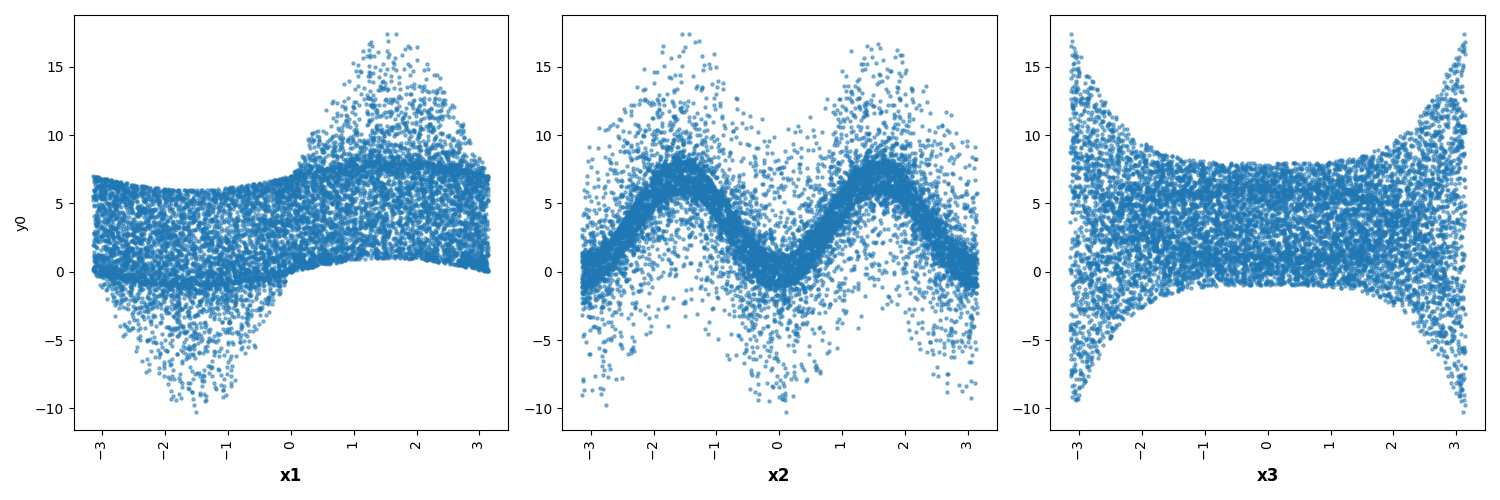
\includegraphics[width=\textwidth]{figures/grid_plot.png}
\caption{Grid plot of input parameters against the model output.}
\label{fig:grid_plot}
\end{figure}

\section{Expectation Convergence Analysis}

The mean estimate convergence analysis examines the expected value of the output temperature as a function of the sample size. The data indicates that as the sample size increases, the mean estimate stabilizes, thus narrowing the confidence interval, which implies the operating range under the specified uncertainty.

Figure \ref{fig:mean_estimate_convergence_plot} illustrates the convergence behavior of the mean estimate, with sample sizes ranging up to 1500. It is observed that the mean estimate initially fluctuates but converges around a stable value near 300.49 K.

\begin{figure}[h]
\centering
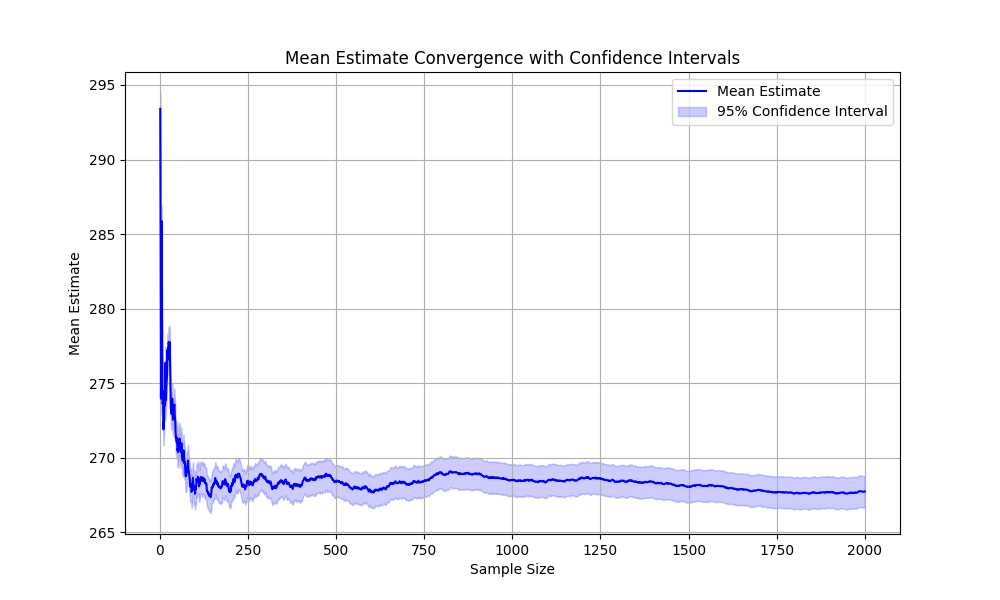
\includegraphics[width=\textwidth]{figures/mean_estimate_convergence_plot.png}
\caption{Mean estimate convergence plot.}
\label{fig:mean_estimate_convergence_plot}
\end{figure}

\section{Sensitivity Analysis}

\subsection{Correlation Coefficients Analysis}

The following table presents the correlation coefficients for the model inputs:

\begin{table}[h]
\centering
\begin{tabular}{|l|c|c|c|c|c|}
\hline
Variable & PCC & Pearson & PRCC & Spearman & SRC & SRRC \\ \hline
radius   & 0.615 & 0.518 & 0.954 & 0.796 & 0.517 & 0.796 \\ \hline
length   & -0.530 & -0.417 & -0.844 & -0.400 & -0.414 & -0.397 \\ \hline
k        & -0.325 & -0.228 & -0.680 & -0.235 & -0.228  & -0.233 \\ \hline
h        & -0.013 & -0.023 & -0.003 & -0.019 & -0.009 & -0.001 \\ \hline
Q        & 0.366 & 0.261 & 0.766 & 0.298 & 0.261 & 0.300 \\ \hline
\end{tabular}
\caption{Correlation coefficients for model inputs.}
\end{table}

As depicted in Figure \ref{fig:correlation_coefficients}, PRCC and SRRC coefficients are generally higher, indicating stronger monotonic relationships as compared to linear correlations.

\begin{figure}[h]
\centering
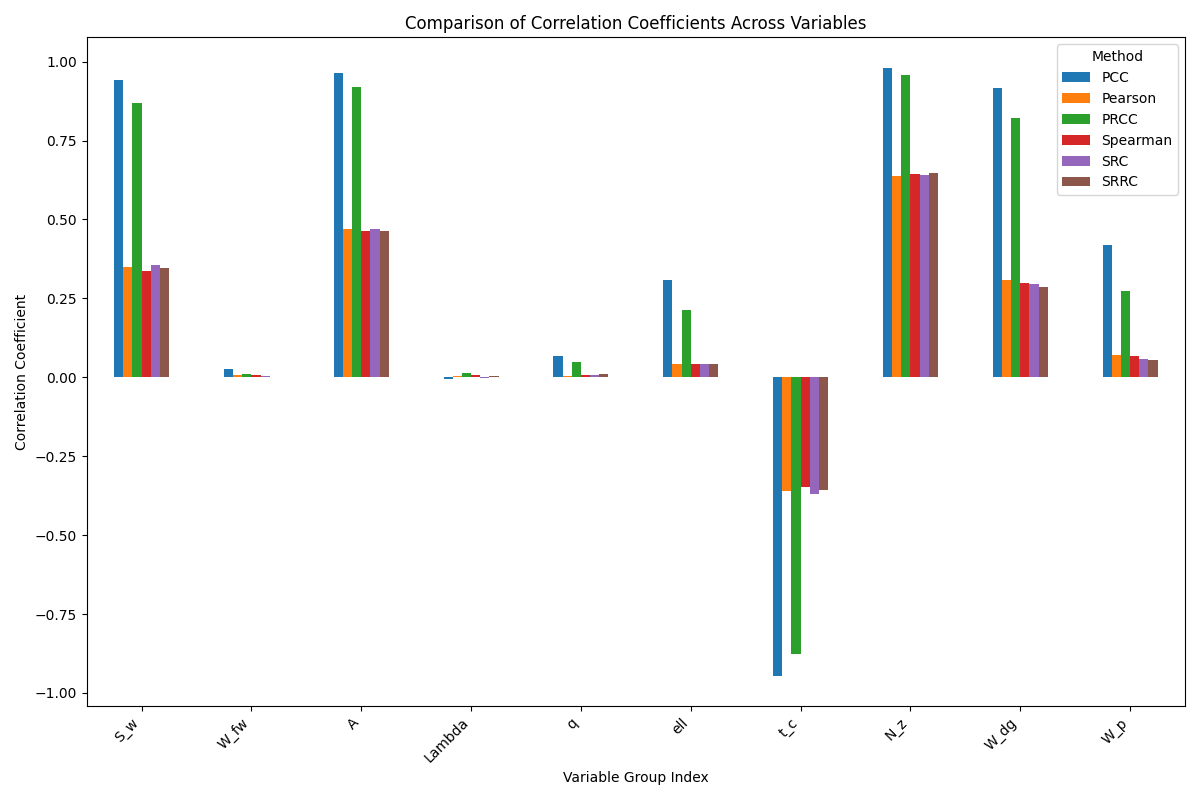
\includegraphics[width=\textwidth]{figures/correlation_coefficients.png}
\caption{Correlation coefficients plot.}
\label{fig:correlation_coefficients}
\end{figure}

\subsection{Sobol' Indices Analysis}

Sobol' indices provide a variance-based sensitivity analysis, highlighting both first-order effects and interaction effects among input parameters. The first-order Sobol' indices indicate the contribution of each input to the output variance, while total-order indices account for both individual and interaction effects.

Tables \ref{tab:sobol_first_order} and \ref{tab:sobol_total_order} present the Sobol' indices for both first-order and total-order effects.

\begin{table}[h]
\centering
\begin{tabular}{|l|c|c|c|}
\hline
Inputs   & Sobol Index & Upper Bound & Lower Bound \\ \hline
radius   & 0.329       & 0.448       & 0.209       \\ \hline
length   & 0.189       & 0.302       & 0.079       \\ \hline
k        & 0.004       & 0.054       & -0.054      \\ \hline
h        & -0.025      & 0.030       & -0.088      \\ \hline
Q        & 0.034       & 0.100       & -0.009      \\ \hline
\end{tabular}
\caption{First-order Sobol' indices for model inputs.}
\label{tab:sobol_first_order}
\end{table}

\begin{table}[h]
\centering
\begin{tabular}{|l|c|c|c|}
\hline
Inputs   & Sobol Index & Upper Bound & Lower Bound \\ \hline
radius   & 0.493       & 1.000       & 0.025       \\ \hline
length   & 0.448       & 0.816       & 0.140       \\ \hline
k        & 0.181       & 0.470       & -0.064      \\ \hline
h        & 0.002       & 0.374       & -0.303      \\ \hline
Q        & 0.283       & 0.582       & 0.006       \\ \hline
\end{tabular}
\caption{Total-order Sobol' indices for model inputs.}
\label{tab:sobol_total_order}
\end{table}

\begin{figure}[h]
\centering
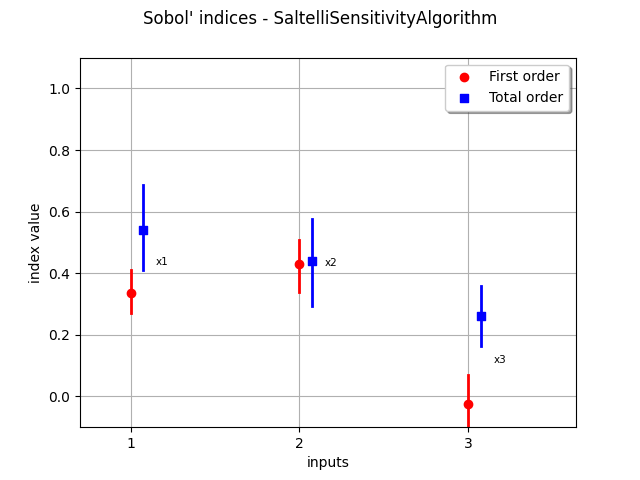
\includegraphics[width=\textwidth]{figures/sobol_indices.png}
\caption{Sobol' indices plot.}
\label{fig:sobol_indices}
\end{figure}

Comparison of correlation coefficients and Sobol' indices reveals consistent sensitivity patterns, with radius and length having significant impacts on the output variability. The Sobol' method’s variance-based approach offers a more nuanced understanding, capturing interaction effects that correlation coefficients might miss.

\section{Key Findings}

Key observations from the analysis include:
- The radius and length significantly impact the model output, both independently and through interactions.
- Parameters such as $k$ and $h$ have minimal impact, likely due to their roles in thermal conduction and convection being secondary to the primary heat generation.
- Negative correlation coefficients for $length$ and $k$ indicate inverse relationships with the output temperature, affirmed by their physical roles in heat dissipation.
- The relatively high PRCC values underscore significant monotonic relationships for key parameters.

\section{Conclusion}

Further refinement should focus on controlling the radius and length for precise thermal management. Parameters with minimal influence, such as $h$, may be deprioritized in sensitivity-driven optimizations.

\section{Summary and Insights for Decision Making}

Understanding the critical influence of key parameters—radius and length—is crucial for effective thermal management. Decision-makers should aim to stabilize these parameters to mitigate variability in thermal outcomes. The analysis demonstrates the utility of both correlation coefficients and variance-based Sobol' indices in identifying and quantifying parameter influences, providing a robust framework for targeted interventions and process optimization.

\end{document}
```
\end{document}